%!TEX root = main.tex


\section{Variables and Probability Models}\label{sec:vague_variables}

\subsection{Probability distributions, Markov kernels and string diagrams}

We make extensive use of probability theory, and the following is a brief introduction to the string diagram notation we use for probabilistic reasoning. This notation comes from the study of Markov categories. Markov categories are abstract categories that represent models of the flow of information. We can form Markov categories from collections of sets -- for example, discrete sets or standard measurable sets -- along with the Markov kernel product as the composition operation. Markov categories come equipped with a graphical language of \emph{string diagrams}, and a coherence theorem which states that calid proofs using string diagrams correspond to valid theorems in \emph{any} Markov category \citep{selinger_survey_2010}. More comprehensive introductions to Markov categories can be found in \citet{fritz_synthetic_2020,cho_disintegration_2019}. Thus, while we limit ourselves to discrete sets in this paper, any derivation that uses only string diagrams is more broadly appliccable.

We say, given a variable $\RV{X}:\Omega\to X$, a probability distribution $\prob{P}^{\RV{X}}$ is a probability measure on $(X,\sigalg{X})$. Recall that a probability measure is a $\sigma$-additive function $\prob{P}^{\RV{X}}:\sigalg{X}\to [0,1]$ such that $\prob{P}^{\RV{X}}(\emptyset)=0$ and $\prob{P}^{\RV{X}}(X)=1$. Given a second variable $\RV{Y}:\Omega\to Y$, a conditional probability $\prob{Q}^{\RV{X}|\RV{Y}}$ is a Markov kernel $\prob{Q}^{\RV{X}|\RV{Y}}:X\kto Y$which is a map $Y\times \sigalg{X}\to [0,1]$ such that

\begin{enumerate}
	\item $y\mapsto \prob{Q}^{\RV{X}|\RV{Y}}(A|y)$ is $\sigalg{B}$-measurable for all $A\in \sigalg{X}$
	\item $A\mapsto \prob{Q}^{\RV{X}|\RV{Y}}{K}(A|y)$ is a probability measure on $(X,\sigalg{X})$ for all $y\in Y$
\end{enumerate}

In the context of discrete sets, a probability distribution can be defined as a vector, and a Markov kernel a matrix.

\begin{definition}[Probability distribution (discrete sets)]
A probability distribution $\prob{P}$ on a discrete set $X$ is a vector $(\prob{P}(x))_{x\in X}\in [0,1]^{|X|}$ such that $\sum_{x\in X} \prob{P}(x) = 1$. For $A\subset X$, define $\prob{P}(A)=\sum_{x\in A} P(x)$.
\end{definition}

\begin{definition}[Markov kernel (discrete sets)]
A Markov kernel $\prob{K}:X\kto Y$ is a matrix $(\prob{K}(y|x))_{x\in X,y\in Y}\in [0,1]^{|X||Y|}$ such that $\sum_{y\in Y} \prob{K}(y|x)=1$ for all $x\in X$. For $B\subset Y$ define $\prob{K}(B|x)=\sum_{y\in B}\prob{K}(y|x)$.
\end{definition}

In the graphical language, Markov kernels are drawn as boxes with input and output wires, and probability measures (which are kernels with the domain $\{*\}$) are represented by triangles:

\begin{align}
\kernel{K}&:=\begin{tikzpicture}[baseline={([yshift=-.5ex]current bounding box.center)}]
	\path (0,0) node (A) {}
	++ (0.5,0) node[kernel] (K) {$\kernel{K}$}
	++ (0.5,0) node (B) {};
	\draw (A) -- (K) -- (B);
\end{tikzpicture}\\
\kernel{P}&:= \begin{tikzpicture}[baseline={([yshift=-.5ex]current bounding box.center)}]
	\path (0,0) node[dist] (K) {$\kernel{P}$}
	++ (0.5,0) node (B) {};
	\draw (K) -- (B);
\end{tikzpicture}
\end{align}

Two Markov kernels $\kernel{L}:X\kto Y$ and $\kernel{M}:Y\kto Z$ have a product $\kernel{L}\kernel{M}:X\kto Z$, given in the discrete case by the matrix product $ \kernel{L}\kernel{M}(z|x) = \sum_{y\in Y} \kernel{M}(z|y)\kernel{L}(y|x)$. Graphically, we represent products between compatible Markov kernels by joining wires together:

\begin{align}
	\kernel{L}\kernel{M}:= \begin{tikzpicture}[baseline={([yshift=-.5ex]current bounding box.center)}]
	\path (0,0) node (A) {$X$}
	++ (0.5,0) node[kernel] (K) {$\kernel{K}$}
	++ (0.7,0) node[kernel] (M) {$\kernel{M}$}
	++ (0.5,0) node (B) {$Z$};
	\draw (A) -- (K) -- (M) -- (B);
\end{tikzpicture}
\end{align}

The Cartesian product $X\times Y:=\{(x,y)|x\in X, y\in Y\}$. Given kernels $\kernel{K}:W\kto Y$ and $\kernel{L}:X\kto Z$, the tensor product $\kernel{K}\otimes\kernel{L}:W\times X\kto Y\times Z$ given by $(\kernel{K}\otimes\kernel{L})(y,z|w,x):=K(y|w) L(z|x)$. The tensor product is graphically represeted by drawing kernels in parallel:

\begin{align}
	\kernel{K}\otimes \kernel{L}&:=\begin{tikzpicture}[baseline={([yshift=-.5ex]current bounding box.center)}]
	\path (0,0) node (A) {$W$}
	++ (0.5,0) node[kernel] (K) {$\kernel{K}$}
	++ (0.5,0) node (B) {$Y$};
	\path (0,-0.5) node (C) {$X$}
	++ (0.5,0) node[kernel] (L) {$\kernel{L}$}
	++ (0.5,0) node (D) {$Z$};
	\draw (A) -- (K) -- (B);
	\draw (C) -- (L) -- (D);
\end{tikzpicture}
\end{align}

We read diagrams from left to right (this is somewhat different to \citet{fritz_synthetic_2020,cho_disintegration_2019,fong_causal_2013} but in line with \citet{selinger_survey_2010}), and any diagram describes a set of nested products and tensor products of Markov kernels. There are a collection of special Markov kernels for which we can replace the generic ``box'' of a Markov kernel with a diagrammatic elements that are visually suggestive of what these kernels accomplish.

The identity map $\text{id}_X:X\kto X$ defined by $(\text{id}_X)(x'|x)= \llbracket x = x' \rrbracket$, where the Iverson bracket $\llbracket \cdot \rrbracket$ evaluates to $1$ if $\cdot$ is true and $0$ otherwise, is a bare line:

\begin{align}
	\mathrm{id}_X&:=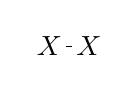
\begin{tikzpicture}[baseline={([yshift=-.5ex]current bounding box.center)}]
	\path (0,0) node (A) {$X$} ++ (0.5,0) node (B) {$X$};
	\draw (A) -- (B);
\end{tikzpicture}
\end{align}

We choose a particular 1-element set $\{*\}$ that acts as the identity in the sense that $\{*\}\times A\cong A\times \{*\} \cong A$ for any set $A$. The erase map $\text{del}_X:X\kto \{*\}$ defined by $(\text{del}_X)(*|x) = 1$ is a Markov kernel that ``discards the input''. It is drawn as a fuse:

\begin{align}
	\text{del}_X&:=\begin{tikzpicture}[baseline={([yshift=-.5ex]current bounding box.center)}]
	\path (0,0) ++ (1,0) node (B) {$X$};
	\draw[-{Rays[n=8]}] (A) -- (B);
\end{tikzpicture}
\end{align}

The copy map $\text{copy}_X:X\kto X\times X$ defined by $(\text{copy}_X)(x',x''|x)=\llbracket x=x' \rrbracket \llbracket x=x'' \rrbracket$ is a Markov kernel that makes two identical copies of the input. It is drawn as a fork:

\begin{align}
	\text{copy}_X&:=\begin{tikzpicture}[baseline={([yshift=-.5ex]current bounding box.center)}]
	\path (0,0) node (A) {$X$} 
	++ (0.5,0) node[copymap] (copy0) {}
	++ (0.5,0.15) node (B) {$X$}
	+ (0,-0.3) node (C) {$X$};
	\draw (A) -- (copy0) to [out=45,in=180] (B) (copy0) to [out=-45, in=180] (C);
\end{tikzpicture}
\end{align}

The swap map $\text{swap}_{X,Y}:X\times Y\kto Y\times X$ defined by $(\text{swap}_{X,Y})(y',x'|x,y)=\llbracket x=x' \rrbracket\llbracket y=y' \rrbracket$ swaps two inputs, and is represented by crossing wires:

\begin{align}
	\text{swap}_X &:=  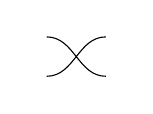
\begin{tikzpicture}[baseline={([yshift=-.5ex]current bounding box.center)}]
		\path (0,0) node (A) {} 
		+ (0,-0.5) node (B) {}
		++ (1,0) node (C) {}
		+ (0,-0.5) node (D) {};
		\draw (A) to [out=0,in=180] (D) (B) to [out=0, in=180] (C);
	\end{tikzpicture}
\end{align}

Because we anticipate that the graphical notation will be unfamiliar, we will include some examples in the next section.

\subsubsection{Examples}

When translating string diagram notation to integral notation, a number of identities can speed up the process.

For arbitrary $\kernel{K}:X\times Y\to Z$, $\kernel{L}:W\to Y$

\begin{align}
 [(\text{id}_X\otimes \kernel{L})\kernel{K}](A|x,w) &= \int_{Y}\int_X   \kernel{K}(z|x',y')\kernel{L}(dy'|w)\text{id}_X(dx'|x)\\
										   &= \int_Y  \kernel{K}(z|x,y') \kernel{L}(dy'|w)
\end{align}

That is, an identity map passes its input to the next kernel in the product. 

For arbitrary $\kernel{K}: X\times Y\times Y\to Z$ (where we apply the above shorthand in the first line):

\begin{align}
 [(\text{id}_X\otimes \text{copy}_Y)\kernel{K}](A|x,y) &= \int_Y\int_Y \kernel{K}(A|x,y',y'') \text{copy}_Y(dy'\times dy''|y)\\
										   &= \kernel{K}(A|x,y,y)
\end{align}

That is, the copy map passes along two copies of its input to the next kernel in the product. 

For a collection of kernels $\kernel{K}^n:Y^n\to Z$, $n\in[n]$, define $(y)^{n}=(y|i\in[n])$ and:

\begin{align}
	\text{copy}^n_Y &:= \begin{cases}
	\text{copy}^{n-1}_Y(\text{id}_{Y^{n-2}}\otimes \text{copy}_Y) & n>2\\
	\text{copy}_Y & n=2
	\end{cases}\\
	(\text{copy}^2_Y\kernel{K}^2)(z|y) &= \kernel{K}^2(z|y,y)\\
\end{align}

Suppose for induction
\begin{align}
(\text{copy}^{n-1}_Y\kernel{K}^{n-1})(z|y) &= \kernel{K}^{n-1}(z|(y)^{n-1})
\end{align}

then
\begin{align}
(\text{copy}^n_Y\kernel{K}^n)(z|y) &= (\text{copy}^{n-1}_Y(\text{id}_{Y^{n-2}}\otimes \text{copy}_Y)\kernel{K}^n)(z|y)\\
									 &= \sum_{y'\in Y^{n-1}}(\text{id}_{Y^{n-2}}\otimes \text{copy}_Y)(\mathbf{y}'|(y)^{n-1})\kernel{K}^n(z|\mathbf{y}')\\
									 &= \kernel{K}^n(z|(y)^n)
\end{align}

That is, we can define the $n$-fold copy map that passes along $n$ copies of its input to the next kernel in the product.

\subsubsection{Example: comb insertion}

The following examples illustrate 2-combs and the insertion operation, both of which we will define later. As an example in translating diagrams, we show how the diagrams for a 2-comb and 2-comb with an inserted Markov kernel can be translated to integral notation.

Consider the Markov kernels $\kernel{K}:W\kto X$, $\kernel{L}:X\times W\times Y\kto Z$ and the 2-comb $\kernel{M}:W\times Y\kto X\times Z$ defined as

\begin{align}
	\kernel{M} = \tikzfig{2_comb}\label{eq:2comb_M}
\end{align}

Following the rules above, we can translate this to ordinary notation by first breaking it down into products and tensor products, and then evaluating these products

\begin{align}
	\kernel{M}(A\times B|w,y) = [&(\text{copy}_W\otimes \text{id}_Y)(\kernel{K}\otimes \text{id}_{W\times Y})\\
	&(\text{copy}_X\otimes \text{id}_{W\times Y})(\text{id}_X\otimes\kernel{L})](A\times B|w,y)\\
						= [&(\kernel{K}\otimes \text{id}_{W\times Y})(\text{copy}_X\otimes \text{id}_{W\times Y})\\
						&(\text{id}_X\otimes\kernel{L})](A\times B|w,w,y)\\
						= \;&\int_{X}  (\text{id}_X\otimes\kernel{L})(A\times B|x',w,y) \kernel{K} (dx'|w)
						](y,z|y',x)\\
						= \;&\int_X \text{id}_X(A|x') \kernel{L}(B|x',w,y)\kernel{K}(dx'|w)\\
						= \;&\int_A \kernel{L}(B|x',w,y)\kernel{K}(dx'|w)
\end{align}

If we are given additionally $\kernel{J}:X\times W\kto Y$, we can define a new Markov kernel $\kernel{N}:W\kto Z$ given by ``inserting'' $\kernel{J}$ into $\kernel{M}$:

\begin{align}
	\kernel{N} = \tikzfig{2comb_inserted_anon}\label{eq:2comb_winsert}
\end{align}


We can translate Equation \ref{eq:2comb_winsert} to

\begin{align}
	\kernel{N}(A\times B\times C|w) = &[\text{copy}_W(\kernel{K}\text{copy}^3_Y\otimes \text{id}_W)\\
	&(\text{id}_Y\otimes\kernel{J}\otimes \text{id}_Y)(\text{id}_Y \otimes \text{copy}_X\otimes \text{id}_Y)\\
	&(\kernel{L}\otimes \text{id}_X\otimes \text{id}_Y)] (A\times B\times C|w)\\
					= &[(\kernel{K}\text{copy}^3_Y\otimes \text{id}_W)(\text{id}_Y\otimes\kernel{J}\otimes \text{id}_Y)\\
					&(\text{id}_Y \otimes \text{copy}_X\otimes \text{id}_Y)\\
					&(\kernel{L}\otimes \text{id}_X\otimes \text{id}_Y)] (A\times B\times C|w,w)\\
					= &\int_X\int_Y\kernel{L}(C|x',w,y') \text{id}_X(A|x') \text{id}_Y(B|y') \kernel{J}(dy'|x',w)\kernel{K}(dx'|w)\\
					= &\int_A\int_B\kernel{L}(C|x',w,y') \kernel{J}(dy'|x',w)\kernel{K}(dx'|w)
\end{align}
\subsection{Semantics of observed and unobserved variables}\label{sec:variables}

We are interested in constructing \emph{probabilistic models} which explain some part of the world. In a model, variables play the role of ``pointing to the parts of the world the model is explaining''. Both observed an unobserved variables play important roles in causal modelling and we think it is worth clarifying what variables of either type refer to. Our approach is a standard one: a probabilistic model is associated with an experiment or measurement procedure that yields values in a well-defined set. Observable variables are obtained by applying well-defined functions to the result of this total measurement. We use a richer sample space that includes ``unobserved variables'' that are formally treated the same way as observed variables, but aren't associated with any real-world counterparts.

Consider Newton's second law in the form $\proc{F}=\proc{MA}$ as a simple example of a model that relates variables $\proc{F}$, $\proc{M}$ and $\proc{A}$. As \citet{feynman_feynman_1979} noted, this law is incomplete -- in order to understand it, we must bring some pre-existing understanding of force, mass and acceleration as independent things. Furthermore, the nature of this knowledge is somewhat perculiar. Acknowledging that physicists happen to know a great deal about forces on an object, it remains true that in order to actually say what the net force on a real object is, even a highly knowledgeable physicist will still have to go and do some measurements, and the result of such measurements will be a vector representing the net forces on that object.

This suggests that we can think about ``force'' $\proc{F}$ (or mass or acceleration) as a kind of procedure that we apply to a particular real world object and which returns a mathematical object (in this case, a vector). We will call $\proc{F}$ a \emph{procedure}. Our view of $\proc{F}$ is akin to \citet{menger_random_2003}'s notion of variables as ``consistent classes of quantities'' that consist of pairing between real-world objects and quantities of some type. Force $\proc{F}$ itself is not a well-defined mathematical thing, as measurement procedures are not mathematically well-defined. At the same time, the set of values it may yield \emph{are} well-defined mathematical things.

We will assume that any procedure will eventually yield an unambiguous value in a defined mathematical set. No actual procedure can be guaranteed to have this property -- any apparatus, however robust, could suffer catastrophic failure -- but we assume that we can study procedures reliable enough that we don't lose much by making this assumption. This assumption allows us to say a procedure $\proc{B}$ yields values in $B$. $\proc{B}\yields x$ is the proposition that $\proc{B}$, when completed, yields the value $x\in B$, and by assumption exactly one of these propositions is true. For $A\subset B$, $\proc{B}\yields A$ is the proposition $\lor_{x\in A} \proc{B}\yields x$. Two procedures $\proc{B}$ and $\proc{C}$ are the same if $\proc{B}\yields x\iff \proc{C}\yields x$ for all $x\in B$. 

The notion of ``yielding values'' allows us to define an operation akin to function composition. If I have a procedure $\proc{B}$ that takes values in some set $B$, and a function $f:B\to C$, define the ``composition'' $f\circ \proc{B}$ to be the procedure $\proc{C}$ that yields $f(x)$ whenever $\proc{B}$ yields $x$. For example, $\proc{MA}$ is the composition of $h:(x,y)\mapsto xy$ with the procedure $(\proc{M},\proc{A})$ that yields the mass and acceleration of the same object. Composition is associative - for all $x\in B$: 

\begin{align}
	(g\circ f)\circ\proc{B}\text{ yields } x &\iff B\text{ yields } (g\circ f)^{-1}(x) \\
	&\iff B\text{ yields } f^{-1}(g^{-1}(x))\\
	&\iff f\circ B \text{ yields } g^{-1}(x)\\
	&\iff g\circ(f\circ B)\text{ yields } x
\end{align}


One might whether there is also some kind of ``append'' operation that takes a standalone $\proc{M}$ and a standalone $\proc{A}$ and returns a procedure $(\proc{M},\proc{A})$. Unlike function composition, this would be an operation that acts on two procedures rather than a procedure and a function. Rather than attempt to define any operation of this type, we simply assume that somehow a procedure has been devised that measures everything of interest, which we will call $\proc{S}$ which takes values in $\Psi$. We assume $\proc{S}$ is such that any procedure of interest can be written as $f\circ \proc{S}$ for some $f$.

For the model $\proc{F}=\proc{MA}$, for example, we could assume $\proc{F}=f\circ \proc{S}$ for some $f$ and $(\proc{M},\proc{A})=g\circ \proc{S}$ for some $g$. In this case, we can get $\proc{MA}=h\circ(\proc{M},\proc{A})=(h\circ g)\circ\proc{S}$. Note that each procedure is associated with a unique function with domain $\Psi$.

Thus far, $\Psi$ is a ``sample space'' that only contains observable variables. To include unobserved variables, we posit a richer sample space $\Omega$ such that the measurement $\proc{S}$ determines an element of some partition of $\Omega$ rather than an element of $\Omega$ itself. Then, by analogy to procedures defined with respect to $\proc{S}$, we identify variables in general with measurable functions defined on the domain $\Omega$. 

Specifically, suppose $\proc{S}$ takes values in $\Psi$. Then we can propose a sample space $\Omega$ such that $|\Omega|\geq |\Psi|$ and a surjective function $\RV{S}:\Omega\to \Psi$ associated with $\proc{S}$. We connect $\Omega$, $\RV{S}$ and $\proc{S}$ with the notion of \emph{consistency with obseravation}:

\begin{align}
 &\omega\in \Omega\text{ is \emph{consistent with observation} iff the result yielded by }\proc{S}\text{ is equal to }\RV{S}(\omega)\label{def:observable}
\end{align}

Thus the procedure $\proc{S}$ eventually restricts the observationally consistent elements of $\Omega$. If $\proc{S}$ yield the result $s$, then the consistent values of $\Omega$ will be $\RV{S}^{-1}(s)$.

One thing to note in this setup is that two different sets of measurement outcomes $\Psi$ and $\Psi'$ entail a different mesurement procedures $\proc{S}$ and $\proc{S}'$, but different sample spaces $\Omega$ and $\Omega'$ may be used to model a single procedure $\proc{S}$. We will sometimes consider different models of the same observable procedures.

As far as we know, distinguishing variables from procedures is somewhat nonstandard, but it is a useful distinction to make. While they may not be explicitly distinguished, both variables and procedures are often discussed in statistical texts. For example, \citet{pearl_causality:_2009} offers the following two, purportedly equivalent, definitions of variables:
\begin{quote}
By a \emph{variable} we will mean an attribute, measurement or inquiry that may take on one of several possible outcomes, or values, from a specified domain. If we have beliefs (i.e., probabilities) attached to the possible values that a variable may attain, we will call that variable a random variable.
\end{quote}

\begin{quote}
This is a minor generalization of the textbook definition, according to which a random variable is a mapping from the sample space (e.g., the set of elementary events) to the real line. In our definition, the mapping is from the sample space to any set of objects called ``values,'' which may or may not be ordered.
\end{quote}

Our view is that the first definition is a definition of a procedure, while the second is a definition of a variable. Variables model procedures, but they are not the same thing. We can establish this by noting that, under our definition, every procedure of interest -- that is, all procedures that can be written $f\circ \proc{S}$ for some $f$ -- is modeled by a variable, but there may be variables defined on $\Omega$ that do not factorise through $\proc{S}$, and these variables do not model procedures.

\subsection{Events}

To recap, we have a procedure $\proc{S}$ yielding values in $\Psi$ that measures everything we are interested in, a sample space $\Omega$ and a function $\RV{S}$ that models $\proc{S}$ in the sense of Definition \ref{def:observable}. We assume also that $\Psi$ has a $\sigma$-algebra $\sigalg{E}$ (this may be the power set of $\Psi$, as measurement procedures are typically limited to finite precision). $\Omega$ is equipped with a $\sigma$-algebra $\sigalg{F}$ such that $\sigma(\RV{S})\subset \sigalg{F}$. If a procedure $\proc{X}=f\circ \RV{S}$ then we define $\RV{X}:\Omega\to X$ by $\RV{X}:=f\circ\RV{S}$.

If a particular procedure $\proc{X}=f\circ \proc{S}$ eventually yields a value $x$, then the values of $\Omega$ consistent with observation must be a subset of $\RV{X}^{-1}(x)$. We define an \emph{event} $\RV{X}\yields x:\equiv \RV{X}^{-1}(x)$, which we read ``the event that $\RV{X}$ yields x''. An event $\RV{X}\yields x$ occurs if the consistent values of $\Omega$ are a subset of $\RV{X}\yields x$, thus ``the event that $\RV{X}$ yields x occurs$\equiv \proc{X}$ yields $x$''. The definition of events applies to all types of variables, not just observables, but we only provide an interpretation of events ``occurring'' when the variable $\RV{X}$ is associated with some $\proc{X}$.

For measurable $A\in \sigalg{X}$, $\RV{X}\yields A=\bigcup_{x\in A} \RV{X}\yields x$. 

Given $\RV{Y}:\Omega\to X$, we can define an append operation for variables: $(\RV{X},\RV{Y}):=\omega\mapsto (\RV{X}(\omega),\RV{Y}(\omega))$. $(\RV{X},\RV{Y})$ has the property that $(\RV{X},\RV{Y})\yields (x,y)= \RV{X}\yields x\cap \RV{Y}\yields y$, which supports the interpretation of $(\RV{X},\RV{Y})$ as the values yielded by $\RV{X}$ and $\RV{Y}$ together.

It is common to use the symbol $=$ instead of $\bowtie$, but we want to avoid this because $\RV{Y}=y$ already has a meaning, namely that $\RV{Y}$ is a constant function everywhere equal to $y$. 

\subsection{Probabilistic models for causal inference}

The sample space $(\Omega,\sigalg{F})$ along with our collection of variables is a ``model skeleton'' -- it tells us what kind of data we might see. The process $\proc{S}$ which tells us which part of the world we're interested in is related to the model $\Omega$ and the observable variables by the criterion of \emph{consistency with observation}. The kind of problem we are mainly interested in here is one where we make use of data to help make decisions under uncertainty. Probabilistic models have a long history of being used for this purpose, and our interest here is in constructing probabilistic models that can be attached to our variable ``skeleton''. 

For causal inference, we find we need to generalise the standard approach to constructing probability models on a given sample space $(\Omega,\sigalg{F})$. The key things we need to handle are \emph{gaps} in our model. \citet{hajek_what_2003} defines \emph{probability gaps} as propositions that do not have a probability assigned to them. Our view of probability gaps is slightly different -- in this work, a model with probability gaps as one that is missing some key parts. If we complete such a model with parts of the appropriate type, we get a standard probability model.

Probability gaps are useful in models used for decision making because, when I have a number of different options I could choose, a model can only help select from them if it tells me what is likely to happen for each choice I could make. Thus if we have a variable representing choices, we must have a model that can tolerate a probability gap for this variable.

As an initial example of a probability gap in causal inference, we will consider the example of truncated factorisation. For this example, we will assume that the reader is familiar enough with marginal probabilities, conditional probabilities and causal models to follow along. We will offer more careful definitions of terms later.

Suppose we have a causal Bayesian network $(\prob{P}^{\RV{XYZ}},\mathcal{G})$ where $\RV{X}:\Omega\to X$, $\RV{Y}:\Omega\to Y$ and $\RV{Z}:\Omega\to Z$ are variables, $\prob{P}^{\RV{XYZ}}$ is a probability measure on $X\times Y\times Z$ that we call ``a probability model of $(\RV{X},\RV{Y},\RV{Z})$'' and $\mathcal{G}$ is a Directed Acyclic Graph whose vertices we identify with $\RV{X}$, $\RV{Y}$ and $\RV{Z}$ that contains the edges $\RV{X}\longrightarrowRHD \RV{Y}$ and $\RV{X}\longleftarrowRHD \RV{Z} \longrightarrowRHD \RV{Y}$. ``Setting $\RV{X}$ to $x$'' is an operation that takes as inputs $\prob{P}^{\RV{XYZ}}$, $\mathcal{G}$ and some $x\in X$ and returns a new probability measure $\prob{P}_x^{\RV{XYZ}}$ on $X\times Y\times Z$ given by \citep[page ~24]{pearl_causality:_2009}:
\begin{align}
	\prob{P}^{\RV{XYZ}}_{x}(x',y,z)=\prob{P}^{\RV{Y|XZ}}(y|x,z)\prob{P}^{\RV{Z}}(z)\llbracket x=x' \rrbracket\label{eq:truncated_fac}
\end{align}

Equation \ref{eq:truncated_fac} embodies three assumptions about a model of the operation of ``setting $\RV{X}$ to $x$''. First, such a model must assign probability 1 to the proposition that $\RV{X}$ yields $x$. Second, such a model must assign the same marginal probability distribution to $\RV{Z}$ as the input distribution; $\prob{P}^{\RV{Z}}=\prob{P}_{x}^{\RV{Z}}$. Finally, our model must also assign the same conditional probability to $\RV{Y}$ given $\RV{X}$ and $\RV{Z}$; $\prob{P}^{\RV{Y}|\RV{XZ}}=\prob{P}_x^{\RV{Y}|\RV{XZ}}$.

Notice that the map $x\mapsto \prob{P}^{\RV{XYZ}}_x$ itself ``looks like'' a conditional probability. It maps each $x\in X$ to a probability distribution over $(\RV{X},\RV{Y},\RV{Z})$. In fact, a popular alternative notation for $\prob{P}^{\RV{XYZ}}_x$ this map is $\prob{P}^{\RV{XYZ}|do(\RV{X}=x)}$, which is clearly suggestive of an interpretation as a kind of conditional probability. We will take this interpretation seriously: we will posit some variable $\RV{U}$ (which may or may not be observable) and a probabilisitic model $\prob{Q}^{\RV{XYZ}|\RV{U}}:=x\mapsto \prob{P}^{\RV{XYZ}}_x$.

We note that the thing called $do(\RV{X}=x)$ or that we have called $\RV{U}$ is often referred to as an \emph{intervention}. Interventions are often things we can choose to do or not to do. Also, perhaps, we could also consider choosing to do or not do an intervention based on the output of some random process. In this case, we will need a model that can tell us which result we are likely to see for any choice of $\prob{Q}_\alpha^{\RV{U}}$; the distribution of $\RV{U}$ is a \emph{probability gap}.

$\prob{Q}^{\RV{XYZ}|\RV{U}}$, as we have defined it so far, is not quite an ideal candidate for for a gappy probability model. Firstly, because conditional probabilities are arbitrary on sets of measure zero with regard to $\prob{P}^{\RV{XYZ}}$, definition \ref{eq:truncated_fac} can be satisfied by multiple probability distributions that differ in meaningful ways. Suppose $\RV{X}$, $\RV{Y}$ and $\RV{Z}$ are binary, $\prob{P}^{\RV{Z}}(1)=1$ and $\prob{P}(\RV{X}\yields \RV{Z})=1$. Then we can consistently choose $\prob{P}^{\RV{Y|XZ}}(1|0,1)=1$ or $\prob{P}^{\RV{Y|XZ}}(1|0,1)=0$ because $\{0,1\}$ is a measure zero event. However, the first choice gives us  $\prob{P}^{\RV{XYZ}}_{0}(0,1,1)=1$ while the second gives us $\prob{P}^{\RV{XYZ}}_{0}(0,1,1)=0$, which are very different opinions regarding ``the result of setting $\RV{X}$ to $1$''.

Secondly, there may be no probability model at all that satisfies Equation \ref{eq:truncated_fac}. For example, suppose $\RV{X}=f\circ\RV{Z}$ for some $f$. Then we must have $\prob{P}^{\RV{X}}_x(x')=\prob{P}^{\RV{Z}}_x(f^{-1}(x'))$ for any $x$. However, we also have $\prob{P}^{\RV{X}}_x(x')=\llbracket x = x' \rrbracket$ for all $x,x'$ and $\prob{P}^{\RV{Z}}_x=\prob{P}^{\RV{Z}}$ for all $x$. Thus if $\RV{X}$ can more than one value, there is at least one choice of $x$ that cannot simultaneously satisfy these requirements.

This might seem like an absurd model, but an analogous causal graph appears in \citet{shahar_association_2009} where $\RV{Z}=(\RV{H},\RV{W})$, representing a person's height and weight, and $\RV{X}$ represents their body mass index, which is to say $\RV{X}=\frac{\RV{W}}{\RV{H}^2}$. Furthermore, this paper uses this model to argue that body mass index cannot have a causal effect. Such an argument cannot be supported by Equation \ref{eq:truncated_fac} because by that equation there is no probability model corresponding to an intervention on $\RV{X}$.

Our first aim is to offer a more careful theory of probability models with gaps in them, addressing these two shortcomings.

\subsection{Probability gaps}

Probability gap models are probability models that are missing key parts. What this means is that they are functions: provide a ``missing part'' or ``insert'' of the right type and you get a probability model. We also consider higher order gaps; an order 1 gap takes an insert and returns an order 0 gap, which in turn can be completed to a model without gaps. 

We consider in particular functions that are \emph{mixture homomorphic} -- calling a gap model on a mixture of inserts is the same the corresponding mixture of gap models of each insert -- and \emph{insert compatible}, which means that we can recover the insert from the probability model we end up with. This set of functions can be identified with Markov kernels of an appropriate type.

A key consideration with regard to probability gaps is that they are \emph{valid} -- that is, if we provide a valid insert what we end up with is either a probability distribution that can be completed to a probability measure on the sample space $\Omega$, or a valid gap model of lower order.

We will make a substantial simplifying assumption: all sets, including the sample space $\Omega$ and any set of values a variable takes, are discrete sets. That is, they are at most countably infinite and the $\sigma$-algebra of measurable sets is the power set. Because we are working with discrete sets we will by convention call probability measures on set elements: $\prob{P}^{\RV{X}}(x):=\prob{P}^{\RV{X}}(\{x\})$. 

\begin{definition}[Probability space]
A probability space is a triple $(\prob{P}^{\Omega},\Omega,\sigalg{F})$, where $\mu$ is a probability measure on $\sigalg{F}$ which, as stated above, we take to be $\mathscr{P}(\Omega)$. We call $\prob{P}^{\Omega}$ the \emph{base measure}, and the superscript $\Omega$ is a convention we use to name base measures.
\end{definition}

Probability spaces along with random variables can be used to define probability distributions of those random variables. We call such distributions \emph{pushforwards}.

\begin{definition}[Pushforward]
Given a probability space and a random variable $\RV{X}:\Omega\to X$, we can define the probability distribution $\prob{P}^{\RV{X}}:\sigalg{X}\to [0,1]$ of $\RV{X}$ as the \emph{pushforward} of $\prob{P}^{\Omega}$ by $\RV{X}$. Specifically, for any $x\in X$, $\prob{P}^{\RV{X}}(x):=\prob{P}^\Omega(\RV{X}\yields x)$. 
\end{definition}

We can alternatively define the pushforward as a Markov kernel product. Let $\kernel{P}_{\RV{X}|\Omega}:\Omega\kto X$ be the Markov kernel $\kernel{P}_{\RV{X}|\Omega}(x|\omega)\mapsto \llbracket x = \RV{X}(\omega)$. Then
\begin{align}
	\prob{P}^{\RV{X}} = \prob{P}^\Omega\prob{P}^{\RV{X}|\Omega}
\end{align}

Instead of starting with a base measure and pushing it forward to find a probability distribution, we can start with a probability distribution and find base measures that pushforward to that distribution. We call such base measures \emph{completions} of our original distribution.

\begin{definition}[Completion]
Given $\RV{X}:\Omega\to X$, an arbitrary probability distribution $\prob{P}^{\RV{X}}:\sigalg{X}\to [0,1]$ and a sample space $\Omega$, there are typically a number of base measures $\prob{P}^\Omega_\alpha$ such that $\prob{P}^{\RV{X}}=\prob{P}_\alpha^\Omega \prob{P}^{\RV{X}|\Omega}$. We call any $\prob{P}^\Omega_\alpha$ with this property a \emph{completion} of $\prob{P}^{\RV{X}}$.
\end{definition}

\begin{definition}[Validity]
Given $\RV{X}:\Omega\to X$, an arbitrary probability distribution $\prob{P}^{\RV{X}}:\sigalg{X}\to [0,1]$ and a sample space $\Omega$, $\prob{P}^{\RV{X}}$ is valid if it has at least one completion.
\end{definition}

Probability gap models have types, which indicate which kinds of inserts they accept and what kind of model you will get as a result. Types correspond to random variables; for the following suppose any uppercase sans serif letter $\RV{X}$ is a random variable $\Omega\to X$:
\begin{itemize}
	\item An order 0 type $\RV{X}$ probability gap model is a probability distribution $\prob{P}^{\RV{X}}$ that has at least one completion to a base measure on $\Omega$
	\item An order 1 type $\RV{X};\RV{Y}$ probability gap model takes a valid order 0 $\RV{X}$ gap model and returns an order 0 $(\RV{X},\RV{Y})$ gap model
	\item An order 2 type $\RV{W};\RV{X};\RV{Y};\RV{Z}$ probability gap model takes a valid order 1 $\RV{X};\RV{Y}$ gap model and returns an order 1 $\RV{W};(\RV{X},\RV{Y},\RV{Z})$ gap model
\end{itemize}

We will introduce order 1 gap models as \emph{conditional probabilities} and order 2 gap models as \emph{probability 2-combs}.

\subsection{Order 1 gaps: conditional probabilities}\label{sec:validity_of_gapprob}

We use the term \emph{conditional probability} to describe order 1 gap models. A conditional probability $\prob{P}^{\RV{Y}|\RV{X}}$ is a valid Markov kernel of the appropriate type.

\begin{definition}[Valid conditional probability]\label{def:valid_conditional_prob}
Given $(\Omega,\sigalg{F})$, $\RV{X}:\Omega\to X$, $\RV{Y}:\Omega\to Y$ a \emph{valid conditional probability} $\prob{P}^{\RV{Y}|\RV{X}}$ is a Markov kernel $X\kto Y$ such that it assigns probability 0 to contradictions:
\begin{align}
	\forall y\in Y, x\in X: (\RV{X},\RV{Y})\yields(x,y) = \emptyset \implies \left(\prob{P}^{\RV{Y}|\RV{X}}(y|x) = 0\right) \lor \left(\RV{X}\yields (x) = \emptyset\right)
\end{align}
\end{definition}

We combine order 0 gap models (probability distributions) with order 1 gap models (conditional probabilities) using the ``copy-product'' $\odot$.

\begin{definition}[Copy-product]\label{def:copyproduct}
Given two Markov kernels $\prob{K}:X\kto Y$ and $\prob{L}:Y\times X\kto Z$, define the copy-product $\prob{K}\odot\prob{L}:X\to Y\times Z$ as
\begin{align}
	\prob{K}\odot\prob{L}:&= \text{copy}_X(\prob{K}\otimes \text{id}_X)(\text{copy}_Y\otimes\text{id}_X )(\text{id}_Y \otimes \prob{L})\\
							&= \tikzfig{copy_product}\\
							&\iff\\
	(\prob{K}\odot\prob{L})(y,z|x) &= \prob{L}(z|y,x)\prob{K}(y|x)
\end{align}
\end{definition}

We say a conditional probability $\prob{P}^{\RV{Y}|\RV{X}}$ extends to a probability distribution $\prob{P}_\alpha^{\RV{XY}}$ via $\prob{P}_\alpha^{\RV{X}}$ if $\prob{P}_\alpha^{\RV{X}|*}\odot \prob{P}^{\RV{Y}|\RV{X}*} = \prob{P}_\alpha^{\RV{XY}|*}$. 

If $\prob{P}^{\RV{Y}|\RV{X}}$ extends to a distribution $\prob{Q}^{\RV{XY}}$ then we say $\prob{P}^{\RV{Y}|\RV{X}}$ is a \emph{disintegration} of $\prob{Q}^{\RV{XY}}$. If the choice of disintegration does not matter, we may use the notation $\overline{\prob{Q}}^{\RV{Y}|\RV{X}}$ to refer to a representative element of this set. The overline is to address an undesirable ambiguity: if we had no overline, we could easily write $\prob{Q}^{\RV{Y}|\RV{X}}$ for any $\prob{Q}^{\RV{YX}}$ without first checking if it matters which choice we make. Refer to the discussion above about the non-uniqueness of the left hand side of Equation \ref{eq:truncated_fac} for an example of the problems this can introduce.

Note that our terminology matches a common informal definition of conditional probability $\prob{P}^{\RV{Y}|\RV{X}}$ -- ``a function that give the probability of $\RV{X}$ given a value of $\RV{Y}$''. However, the usual formal definition of ``the'' conditional probability $\prob{P}^{\RV{Y}|\RV{X}}$ defines what we would write $\overline{\prob{P}}^{\RV{Y}|\RV{X}}$ given some $\prob{P}^{\RV{XY}}$; that is, a representative member of the set of disintegrations of $\prob{P}^{\RV{XY}}$. We choose to call things like $\prob{P}^{\RV{Y}|\RV{X}}$ ``conditional probabilities'' because we think it would be confusing to call them anything else. We refer to \citet{hajek_what_2003} for arguments that our definition is a better match informal usage of this term than the standard definition.

Arbitrary conditional probabilities do not necessarily extend to valid probability distributions. For example, suppose we $X=Y$ and $\RV{X}=\RV{Y}$ and some $\prob{P}^{\RV{Y}|\RV{X}}$ such that, given $x\neq x'\in X$, $\prob{P}^{\RV{Y}|\RV{X}}(x|x')=a>0$. Take $\prob{P}_\alpha^{\RV{X}}(x')=1$ and then $\prob{P}_\alpha^{\RV{XY}}((x',x))=a>0$ also. For every probability model $\prob{Q}^{\RV{I}}\in \Delta(\Omega)$,
\begin{align}
\prob{Q}^{\RV{XY}}(x,x')&=\prob{Q}^{\RV{I}}(\RV{X}\yields x\cap\RV{X}\yields x')\\
&= \llbracket x=x' \rrbracket
\end{align}
Thus $\prob{P}_\alpha^{\RV{XY}}$ is not valid.

The key justification for our definition of validity is that valid conditional probabilities guarantee that we can extend the conditional probability to a base measure. In fact, Definition \ref{def:valid_conditional_prob} is equivalent to defining valid conditional probabilities as those that extend to valid probability distributions, given any valid probability distribution (Theorem \ref{th:valid_conditional_probability}). In addition, the defintion of validity itself is equivalent to Definition \ref{def:valid_conditional_prob} under the identification of probability distributions with trivial conditional probabilities (Theorem \ref{th:valid_agree}).

\begin{theorem}[Agreement of validity criteria for conditional probabilities]\label{th:valid_agree}
Given $\RV{X}:\Omega\to X$, with $\Omega$ and $X$ discrete, a probability $\prob{P}^{\RV{X}}$ is valid if and only if the conditional probability $\prob{P}^{\RV{X}|*}:=*\mapsto \prob{P}^{\RV{X}}$ is valid.
\end{theorem}

\begin{proof}
$*\yields *=\Omega$ necessarily. Thus validity of $\prob{P}^{\RV{X}|*}$ means 

\begin{align}
	\forall x\in X: \RV{X}\yields (x)=\emptyset \implies \prob{P}^{\RV{X}|*}(x|*)&=0\\
	&= \prob{P}^{\RV{X}}(x)\label{eq:nec_and_suff}
\end{align}

If: We refer to \citet{ershov_extension_1975} Theorem 2.5 for the proof that Equation \ref{eq:nec_and_suff} is necessary and sufficient for the existence of $\prob{P}^{\RV{I}}$ such that $\prob{P}^{\RV{I}}(\RV{X}^{-1}(A))=\prob{P}^{\RV{X}}(A)$ for all $A\in \sigalg{X}$ when $(\Omega,\sigalg{F})$ and $(X,\sigalg{X})$ are standard measurable. If $\Omega$ and $X$ are discrete, then they are standard measurable.

Only if: If $\RV{X}\yields x=\emptyset$ then $\prob{P}^{\RV{X}}(x)=\prob{P}^{\RV{I}}(\emptyset)=0$.
\end{proof}


\begin{lemma}[Valid conditional probabilities are validly extendable]\label{lem:valid_extendability}
Given $(\Omega,\sigalg{F})$, $\RV{X}:\Omega\to X$, $\RV{Y}:\Omega\to Y$, $\RV{Z}:\Omega\to Z$ and any valid conditional probabilities $\prob{P}^{\RV{Y}|\RV{X}}$ and $\prob{Q}^{\RV{Z}|\RV{Y}\RV{X}}$, $ \prob{P}^{\RV{Y}|\RV{X}}\odot \prob{Q}^{\RV{Z}|\RV{Y}\RV{X}}$ is also a valid conditional probability.
\end{lemma}

\begin{proof}
Let $\prob{R}^{\RV{YZ}|\RV{X}}:=\prob{P}^{\RV{Y}|\RV{X}}\odot \prob{Q}^{\RV{Z}|\RV{Y}\RV{X}}$.

We only need to check validity in $x\in \RV{X}(\Omega)$, as it is automatically satisfied for other values of $\RV{X}$.

For all $x\in \RV{X}(\Omega)$, $\RV{X}\yields x\cap\RV{Y}\yields y=\emptyset$, $\prob{P}^{\RV{Y}|\RV{X}}(y|x)=0$ by validity. Thus
\begin{align}
	\prob{R}^{\RV{YZ}|\RV{X}}(y,z|x) &= \prob{Q}^{\RV{Z}|\RV{YX}}(z|y,x)\prob{P}^{\RV{Y}|\RV{X}}(y|x)\\
								  &\leq \prob{P}^{\RV{Y}|\RV{X}}(y|x)\\
								  &=0
\end{align}

For all $(x,y)\in (\RV{X},\RV{Y})(\Omega)$, $z\in Z$ such that $(\RV{X},\RV{Y},\RV{Z})\yields (x,y,z)=\emptyset$, $\prob{Q}^{\RV{Z}|\RV{YX}}(z|y,x)=0$ by validity. Thus for any such $(x,y,z)$:
\begin{align}
	\prob{R}^{\RV{YZ}|\RV{X}}(y,z|x) &= \prob{Q}^{\RV{Z}|\RV{YX}}(z|y,x)\prob{P}^{\RV{Y}|\RV{X}}(y|x)\\
								  &=0
\end{align}
\end{proof}

\begin{corollary}[Valid conditional probability is validly extendable to a probability distribution]
Given $\Omega$, $\RV{U}:\Omega\to U$, $\RV{W}:\Omega\to W$ and a valid conditional probability $\prob{T}^{\RV{W}|\RV{U}}$, then for any valid conditional probability $\prob{V}^{\RV{U}}$, $\prob{V}^{\RV{U}}\odot \prob{T}^{\RV{W}|\RV{U}}$ is a valid probability distribution.
\end{corollary}

\begin{proof}
Applying Lemma \ref{lem:valid_extendability} choosing $\RV{X}=*$, $\RV{Y}=\RV{U}$, $\RV{Z}=\RV{W}$ and $\prob{P}^{\RV{Y}|\RV{X}}=\prob{V}^{\RV{U}|*}$ and $\prob{Q}^{\RV{Z}|\RV{YX}}=\prob{T}^{\RV{W}|\RV{U*}}$ we have $\prob{R}^{WU|*}:=\prob{V}^{\RV{U}|*}\odot \prob{T}^{\RV{W}|\RV{U}*}$ is a valid conditional probability. Then $\prob{R}^{\RV{WU}}\cong \prob{R}^{\RV{WU}|*}$ is valid by Theorem \ref{th:valid_agree}.
\end{proof}

\begin{theorem}[Validity of conditional probabilities]\label{th:valid_conditional_probability}
Suppose we have $\Omega$, $\RV{X}:\Omega\to X$, $\RV{Y}:\Omega\to Y$, with $\Omega$, $X$, $Y$ discrete. A conditional probability $\prob{T}^{\RV{Y}|\RV{X}}$ is valid if and only if for all valid probability distributions $\prob{V}^{\RV{X}}$, $\prob{V}^{\RV{X}}\odot \prob{T}^{\RV{Y}|\RV{X}}$ is a valid probability distribution.
\end{theorem}

\begin{proof}
If: this follows directly from Lemma \ref{lem:valid_extendability}.

Only if: suppose $\prob{T}^{\RV{Y}|\RV{X}}$ is invalid. Then there is some $x\in X$, $y\in Y$ such that $\RV{X}\yields(x)\neq \emptyset$, $(\RV{X},\RV{Y})\yields(x,y)=\emptyset$ and $\prob{T}^{\RV{Y}|\RV{X}}(y|x)>0$. Choose $\prob{V}^{\RV{X}}$ such that $\prob{V}^{\RV{X}}(\{x\})=1$; this is possible due to standard measurability and valid due to $\RV{X}^{-1}(x)\neq \emptyset$. Then
\begin{align}
	(\prob{V}^{\RV{X}}\odot \prob{T}^{\RV{Y}|\RV{X}})(x,y) &= \prob{T}^{\RV{Y}|\RV{X}}(y|x) \prob{V}^{\RV{X}}(x)\\
																	 &= \prob{T}^{\RV{Y}|\RV{X}}(y|x)\\
																	 &>0
\end{align}
Hence $\prob{V}^{\RV{X}}\odot \prob{T}^{\RV{Y}|\RV{X}}$ is invalid.
\end{proof}

Given any two conditional probabilities $\prob{T}^{\RV{Y}|\RV{X}}$, $ \prob{U}^{\RV{Y}|\RV{X}}$ such that there is some $x\in \RV{X}(\Omega)$, $A\in \sigalg{Y}$ for which $\prob{T}^{\RV{Y}|\RV{X}}(A|x)\neq \prob{U}^{\RV{Y}|\RV{X}}(A|x)$, there exists some $\prob{Q}^{\RV{X}}$ such that $\prob{Q}^{\RV{X}}\odot \prob{T}^{\RV{Y}|\RV{X}}\neq \prob{Q}^{\RV{X}}\odot \prob{U}^{\RV{Y}|\RV{X}}$. We can see this by letting $\prob{Q}^{\RV{X}}$ assign probability 1 to some value of $x$ on which $\prob{T}^{\RV{Y}|\RV{X}}$ and $\prob{U}^{\RV{Y}|\RV{X}}$ differ. Thus if we are using conditional probability as a probability model with a gap, uniqueness requires that the conditional probability be represented by a Markov kernel that is unique up to the set of impossible values of the conditioning variable. In contrast, conditional probability derived from a standard probability model may be represented by a Markov kernel unique up to a measure zero set, which is a strictly weaker condition because the set of impossible values must be given measure 0 by any valid probability distribution.

We finally note that a conditional probability $\prob{P}^{\RV{Y}|\RV{X}}$ along with the copy-product $\odot$ corresponds precisely to the set of insert compatible mixture homomorphisms.

\begin{definition}[Marginalisation]

\end{definition}

\begin{lemma}[Marginal probabilities are unique compatible submodels]

\end{lemma}

\begin{definition}[Delta notation]

\end{definition}

\begin{definition}[Order 1 insert compatibility]
Given a function $f:\Delta(X)\to \Delta(X\times Y)$, $f$ is \emph{insert-compatible} if
\begin{align}
	\tikzfig{marginal_functions}
\end{align}
\end{definition}

\begin{definition}[Mixture homomorphic]
Given a function $f:\Delta(X)\to \Delta(X\times Y)$, $f$ is \emph{mixture homomorphic} if
\begin{align}
	f(a\prob{P}^{\RV{X}}_1 + (1-a)\prob{P}^{\RV{X}}_2) = af(\prob{P}^{\RV{X}}_1) + (1-a)f(\prob{P}^{\RV{X}}_2)
\end{align}
\end{definition}

\emph{Proposition:} Every insert-compatible, mixture homomorphic function from $\Delta(X)\to \Delta(X\times Y)$ can be identified with a Markov kernel $X\kto X\times Y$.

\emph{Proof sketch:} We can write any probability measure over a discrete space as a mixture of delta-measures. Define $\kernel{K}(x,y|x'):=f(\delta_{x'})(x,y)$. Then
\begin{align}
	f(\mu)(x,y) &= f(\sum_{i\in X}\mu(i)\delta_i)(x,y)\\
			 &= \sum_{i\in X} \mu(i)f(\delta_i)(x,y)\\
			 &= \sum_{i\in X} \mu(i)\kernel{K}(x,y|i)\\
			 &= (\mu \kernel{K})(x,y)
\end{align}

Due to insert compatibility, we also require for some $\kernel{L}\in\Delta(Y)$
\begin{align}
	\sum_y f(\delta_{x'})(x,y) &= \llbracket x=x' \rrbracket\\
	\implies f(\delta_{x'})(x,y) &= \llbracket x=x' \rrbracket\kernel{L}(y|x)
\end{align}

Thus
\begin{align}
	f(\mu) = \mu\odot \kernel{L}
\end{align}

\subsection{Order 2 gaps: probability combs}

An order-2 gap model can be extended with an order-1 gap model to yield an order-1 gap model. Order-2 gap models are \emph{probability 2-combs} \citep{chiribella_quantum_2008,jacobs_causal_2019}.

\begin{definition}[Probability 2-comb]
Given $\RV{W}:\Omega\to W$, $\RV{X}:\Omega\to X$, $\RV{Y}:\Omega\to Y$, $\RV{Z}:\Omega\to Z$, a probability 2-comb $\prob{P}^{\RV{X}|\RV{W}\square\RV{Z}|\RV{Y}}:W\times Y\kto X\times Z$ is a Markov kernel such that for some $\prob{P}^{\RV{X}|\RV{W}}:W\kto X$
\begin{align}
	\tikzfig{2_comb_properdef}
\end{align}
Coupled with the validity conditions
\begin{enumerate}
	\item $\prob{P}^{\RV{X}|\RV{W}}$ is valid as a conditional probability
	\item $(\RV{W},\RV{X},\RV{Y},\RV{Z})\yields(w,x,y,z)=\emptyset$ implies $\prob{P}^{\RV{X}|\RV{W}\square\RV{Z}|\RV{Y}}(x,z|w,y)=0$ or $(\RV{W},\RV{X},\RV{Y})\yields(w,x,y)=\emptyset$
\end{enumerate}
\end{definition}

With discrete sets, and in general wherever we have kernel disintegrations, there exists some $\disint{P}^{\RV{Z}|\RV{WXY}}:W\times X\times Y\kto Z$ (Lemma \ref{lem:disint_exist}) such that
\begin{align}
	\prob{P}^{\RV{X}|\RV{W}\square\RV{Z}|\RV{Y}} &= \tikzfig{probability_2_comb}
\end{align}

We define the operation $\text{insert}$ that takes a 2-comb and a conditional probability and returns a conditional probability.

\begin{align}
	\text{insert}(\prob{P}_\alpha^{\RV{Y}|\RV{XW}},\prob{P}^{\RV{X}|\RV{W}\square\RV{Z}|\RV{Y}}) = \prob{P}^{\RV{X}|\RV{W}}\odot\prob{P}_\alpha^{\RV{Y}|\RV{XW}} \odot \disint{P}^{\RV{Z}|\RV{WXY}}\label{eq:insert}
\end{align}

We can depict this operation graphically in a somewhat informal way as ``inserting'' $\prob{P}_\alpha^{\RV{Y}|\RV{XW}}$ into $\prob{P}^{\RV{X}|\RV{W}\square\RV{Z}|\RV{Y}}$:

\begin{align}
	\text{Insert}\left(\tikzfig{insert_opn2}\right)\\= \tikzfig{2comb_inserted}\label{eq:insert_op}
\end{align}

Just as in Section \ref{sec:validity_of_gapprob}, a key concern for probability 2-combs is \emph{valid extendability}. The insert operation we define for 2-combs is uniquely defined by Equation \ref{eq:insert} (Theorem \ref{th:equiv_insert}, and yields a valid conditional probability given any valid inputs (Theorem \ref{th:extension_2comb_valid}).

\begin{theorem}[Equivalence of 2-comb disintegrations]\label{th:equiv_insert}
Given a 2-comb $\prob{P}^{\RV{X}|\RV{W}\square\RV{Z}|\RV{Y}}$ and any two disintegrations $\disint{P}^{\RV{Z}|\RV{WXY}}_1$, $\disint{P}^{\RV{Z}|\RV{WXY}}_2$, for all valid extensions $\prob{P}_\alpha^{\RV{Y}|\RV{XW}}$
\begin{align}
	\prob{P}^{\RV{X}|\RV{W}}\odot \prob{P}_\alpha^{\RV{Y}|\RV{XW}} \odot \disint{P}^{\RV{Z}|\RV{WXY}}_1 = \prob{P}^{\RV{X}|\RV{W}}\odot \prob{P}_\alpha^{\RV{Y}|\RV{XW}} \odot \disint{P}^{\RV{Z}|\RV{WXY}}_2
\end{align}
\end{theorem}

\begin{proof}
For any $w,x,y,z$

\begin{align}
	(\prob{P}^{\RV{X}|\RV{W}}\odot \prob{P}_\alpha^{\RV{Y}|\RV{XW}} \odot \disint{P}^{\RV{Z}|\RV{WXY}}_1)(x,y,z|w) &= \prob{P}^{\RV{Y}|\RV{WX}}_\alpha(y|w,x)\prob{P}^{\RV{X}|\RV{W}}(x|w)\disint{P}_1^{\RV{Z}|\RV{XYW}}(z|x,y,w)\\
	&= \prob{P}^{\RV{X}|\RV{W}\square\RV{Z}|\RV{Y}}(x,z|w,y)\\
	&= \prob{P}^{\RV{Y}|\RV{WX}}_\alpha(y|w,x)\prob{P}^{\RV{X}|\RV{W}}(x|w)\disint{P}_2^{\RV{Z}|\RV{XYW}}(z|x,y,w)
\end{align}
\end{proof}

\begin{theorem}[Extension of valid probability 2-combs]\label{th:extension_2comb_valid}
Given $\Omega$, $\RV{W}:\Omega\to W$, $\RV{X}:\Omega\to X$, $\RV{Y}:\Omega\to Y$ and $\RV{Z}:\Omega\to Z$, a probability 2-comb $\prob{P}^{\RV{X}|\RV{W}\square\RV{Z}|\RV{Y}}$ is valid if and only if $\text{insert}(\prob{P}_\alpha^{\RV{Y}|\RV{WX}},\prob{P}^{\RV{X}|\RV{W}\square\RV{Z}|\RV{Y}})$ is valid for all valid $\prob{P}_\alpha^{\RV{Y}|\RV{WX}}$.
\end{theorem}

\begin{proof}
Only if:

Note that
\begin{align}
	\prob{P}_\alpha^{\RV{XYZ}|\RV{W}}&:=\text{insert}(\prob{P}_\alpha^{\RV{Y}|\RV{WX}},\prob{P}^{\RV{X}|\RV{W}\square\RV{Z}|\RV{Y}})\\
	\prob{P}_\alpha^{\RV{XYZ}|\RV{W}}(xyz|w) &= \prob{P}^{\RV{Y}|\RV{WX}}_\alpha(y|w,x)\prob{P}^{\RV{X}|\RV{W}}(x|w)\disint{P}^{\RV{Z}|\RV{XYW}}(z|x,y,w)\\
	&= \prob{P}^{\RV{X}|\RV{W}\square\RV{Z}|\RV{Y}}(x,z|w,y)\prob{P}_\alpha(y|x)
\end{align}

Suppose $\prob{P}^{\RV{X}|\RV{W}\square\RV{Z}|\RV{Y}}$ is valid. If $(\RV{W},\RV{X},\RV{Y},\RV{Z})\yields(w,x,y,z)=\emptyset$ then either $\prob{P}^{\RV{X}|\RV{W}\square\RV{Z}|\RV{Y}}(x,z|w,y)=0$ and hence $\prob{P}_\alpha^{\RV{XYZ}|\RV{W}}(xyz|w)=0$ or $(\RV{W},\RV{X},\RV{Y})\yields(w,x,y)=\emptyset$.

If $(\RV{W},\RV{X},\RV{Y})\yields(w,x,y)=\emptyset$ then either $(\RV{W},\RV{X})\yields (w,x)\neq\emptyset$ and by validity $\prob{P}^{\RV{Y}|\RV{WX}}_\alpha(y|w,x)=0$ and so $\prob{P}_\alpha^{\RV{XYZ}|\RV{W}}(xyz|w)=0$ or $(\RV{W},\RV{X})\yields(w,x)=\emptyset$.

If $(\RV{W},\RV{X})\yields(w,x)=\emptyset$ then either $\RV{W}\yields w\neq \emptyset$ and by validity $\prob{P}^{\RV{X}|\RV{W}}(x|w)=0$ and so $\prob{P}_\alpha^{\RV{XYZ}|\RV{W}}(xyz|w)=0$ or $\RV{W}\yields w=\emptyset$, in which case $\prob{P}_\alpha^{\RV{XYZ}|\RV{W}}(xyz|w)$ may take any value.

If:
Suppose $\prob{P}^{\RV{X}|\RV{W}\square\RV{Z}|\RV{Y}}$ is invalid. Then either $\prob{P}^{\RV{X}|\RV{W}}$ is invalid or $\prob{P}^{\RV{X}|\RV{W}\square\RV{Z}|\RV{Y}}(x,z|w,y)>0$ on some $(w,x,y,z)$ such that $(\RV{W},\RV{X},\RV{Y},\RV{Z})\yields(w,x,y,z)= \emptyset$ and $(\RV{W},\RV{X},\RV{Y})\yields(w,x,y)\neq \emptyset$.

Suppose $\prob{P}^{\RV{X}|\RV{W}}$ is invalid. Then

\begin{align}
	\prob{P}_\alpha^{\RV{X}|\RV{W}}(x|w) &= \sum_{y\in Y,z\in Z}\prob{P}_\alpha^{\RV{XYZ}|\RV{W}}(xyz|w)\\
										 &= \prob{P}^{\RV{X}|\RV{W}}(x|w)
\end{align}

Thus $\prob{P}_\alpha^{\RV{X}|\RV{W}}(x|w)$ is invalid and therefore so too is $\prob{P}_\alpha^{\RV{XYZ}|\RV{W}}$.

Suppose we have some $(w,x,y,z)$ such that $(\RV{W},\RV{X},\RV{Y},\RV{Z})\yields(w,x,y,z)= \emptyset$, $(\RV{W},\RV{X},\RV{Y})\yields(w,x,y)\neq \emptyset$ and $\prob{P}^{\RV{X}|\RV{W}\square\RV{Z}|\RV{Y}}(x,z|w,y)>0$.

By supposition, there is a valid $\prob{P}_\alpha^{\RV{Y}|\RV{WX}}$ such that $\prob{P}_\alpha^{\RV{Y}|\RV{WX}}(y|w,x)=1$. Then

\begin{align}
	\prob{P}_\alpha^{\RV{XYZ}|\RV{W}}(xyz|w) &= \prob{P}^{\RV{X}|\RV{W}\square\RV{Z}|\RV{Y}}(x,z|w,y)\prob{P}_\alpha(y|x)\\
											 &= \prob{P}^{\RV{X}|\RV{W}\square\RV{Z}|\RV{Y}}(x,z|w,y)\\
											 &>0
\end{align}
So $\prob{P}_\alpha^{\RV{XYZ}|\RV{W}}$ is invalid.
\end{proof}

It is also the case that if we combine two valid conditional probabilities to form a 2-comb, the result is a valid 2-comb.

\begin{theorem}[Valid conditional probabilities combine to a valid 2-comb]\label{lem:valid_conditionals}
Given valid conditional probabilities $\prob{P}^{\RV{X}|\RV{W}}$ and $\prob{P}^{\RV{Z}|\RV{WXY}}$
\begin{align}
	\tikzfig{probability_2_comb}
\end{align}
Is a valid 2-comb.
\end{theorem}

\begin{proof}
Validity of $\prob{P}^{\RV{X}|\RV{W}}$ is by assumption, and validity of $\prob{P}^{\RV{Z}|\RV{WXY}}$ means $(\RV{W},\RV{X},\RV{Y},\RV{Z})\yields(w,x,y,z)=\emptyset$ implies $\prob{P}^{\RV{Z}|\RV{WXY}}(z|w,x,y)=0$ or $(\RV{W},\RV{X},\RV{Y})\yields(w,x,y)=\emptyset$. This in turn implies $\prob{P}^{\RV{Z}|\RV{WXY}}(z|w,x,y)=0$ or $(\RV{W},\RV{X},\RV{Y})\yields(w,x,y)=\emptyset$.
\end{proof}


\subsection{Revisiting truncated factorisation}

We have established that, at least for discrete sets, probability 2-combs are a general kind of object that maps a conditional probability to a conditional probability. Thus they model choices that correspond to conditional probabilities, rather than probability distributions. We initially considered that a truncated factorisation might be a conditional probability -- that is, it could be used to model choices that correspond to probability distributions of the choice variable $\RV{U}$ that we introduced. If we instead consider the possibility that the model of ``interventions'' that Equation \ref{eq:truncated_fac} is suggesting is actually a probability 2-comb, we find that both of the problems we identified are automatically solved.

Suppose we have a 2-comb $\prob{P}^{\RV{Z}\square\RV{Y}|\RV{X}}$. Then we have some $\prob{P}^{\RV{Z}}$, $\disint{P}^{\RV{Y}|\RV{XZ}}$ unique up to equivalence such that

\begin{align}
	\prob{P}^{\RV{Z}\square\RV{Y}|\RV{X}}(z,y|x) &= \disint{P}^{\RV{Y|XZ}}(y|x,z)\prob{P}^{\RV{Z}}(z)
\end{align}

By Lemma \ref{lem:nocopy2}, we also have

\begin{align}
	\prob{P}^{\RV{Z}\square\RV{XY}|\RV{X}}(z,x',y|x) &= \disint{P}^{\RV{Y|XZ}}(y|x,z)\prob{P}^{\RV{Z}}(z)\llbracket x=x' \rrbracket\label{eq:2comb_cbn}
\end{align}

Compare this to Equation \ref{eq:truncated_fac}, which we reproduce here for convenience:

\begin{align*}
	\prob{P}^{\RV{XYZ}}_{x}(x',y,z)=\prob{P}^{\RV{Y|XZ}}(y|x,z)\prob{P}^{\RV{Z}}(z)\llbracket x=x' \rrbracket
\end{align*}

These equations look almost identical, and suggest an alternative approach to modelling intervention. Instead of \emph{defining} an interventional conditional probability via truncated factorisation, suppose we have an interventional model that is a probability 2-comb, and that satisfies
\begin{align}
	\prob{P}_{\text{obs}}^{\RV{XYZ}} = \text{insert}(\prob{P}_{\text{obs}}^{\RV{X}|\RV{Z}}, \prob{P}^{\RV{Z}\square\RV{XY}|\RV{X}})
\end{align}
For some observational insert $\prob{P}_{\text{obs}}^{\RV{X}|\RV{Z}}$.

Under this view, we cannot necessarily derive $\prob{P}^{\RV{Z}\square\RV{XY}|\RV{X}}$ from the observational probability distribution $\prob{P}_{\text{obs}}^{\RV{XYZ}}$, as we cannot guarantee that any particular $\disint{P}_{\text{obs}}^{\RV{Y}|\RV{XZ}}$ is a representative of $\disint{P}^{\RV{Y}|\RV{XZ}}$. This is as it should be -- if we have meaningfully different choices of $\disint{P}_{\text{obs}}^{\RV{Y}|\RV{XZ}}$ arising from measure zero sets, we cannot decide which one will model interventions without more information. The 2-comb $\prob{P}^{\RV{Z}\square\RV{XY}|\RV{X}}$ itself stands for a unique map from interventions to probability distributions, rather than the potentially large set of different maps of this type.

The second issue we raised was the nonexistence of $\prob{P}^{\RV{XYZ}}_{x}$ if, for example, $\RV{X}=f\circ \RV{Z}$. Because $\prob{P}_{\text{obs}}^{\RV{Z}}$ and $\disint{P}_{\text{obs}}^{\RV{Y}|\RV{XZ}}$ are both valid, Lemma \ref{lem:valid_conditionals} ensures that any 2-comb defined by any choice of these conditional probabilities is also valid, and so Equation \ref{eq:2comb_cbn} defines a valid object. Because we have a 2-comb which is extended by \emph{conditional probabilities} rather than by probability distributions, and these conditional probabilities \emph{must be valid}, we can validly extend $\prob{P}^{\RV{Z}\square\RV{XY}|\RV{X}}$ even when $\RV{X}=f\circ \RV{Z}$ -- it's just that validity requires that any extending conditional must be such that $\prob{P}_\alpha^{\RV{X}|\RV{Z}}(x|z)=\llbracket x=f(z) \rrbracket$.

\todo[inline]{So: 2-combs do what we want truncated factorisation to do without breaking down in edge cases, except maybe when we go to uncountably infinite sets.}

\subsection{Useful results}

\subsubsection{Repeated variables}

Lemmas \ref{lem:nocopy1} and \ref{lem:nocopy2} establish that models of repeated variables must connect the repetitions with a copy map.

\begin{lemma}[Output copies of the same variable are identical]\label{lem:nocopy1}
For any $\Omega$, $\RV{X},\RV{Y},\RV{Z}$ random variables on $\Omega$ and conditional probability $\model{K}^{\RV{YZ}|\RV{X}}$, there is a conditional probability $\kernel{K}^{\RV{YYZ}|\RV{X}}$ unique up to impossible values of $\RV{X}$ such that
\begin{align}
	\tikzfig{kyyz} = \model{K}^{\RV{YZ}|\RV{X}}
\end{align}
and it is given by
\begin{align}
		\kernel{K}^{\RV{YYZ}|\RV{X}} &= \tikzfig{compose_with_copymap}\\
		&\iff \\
		\kernel{K}^{\RV{YYZ}|\RV{X}}(y,y',z|x) &= \llbracket y=y' \rrbracket\kernel{K}^{\RV{YZ}|\RV{X}}(y,z|x)\\
\end{align}
\end{lemma}

\begin{proof}
If we have a valid $\model{K}^{\RV{YYZ}|\RV{X}}$, it must be the pushforward of $(\RV{Y},\RV{Y},\RV{Z})$ under some $\model{K}^{\RV{I}|\RV{X}}$. Furthermore, $\model{K}^{\RV{YZ}|\RV{X}}$ must be the pushforward of $(*,\RV{Y},\RV{Z})\cong (\RV{Y},\RV{Z})$ under the same $\model{K}^{\RV{I}|\RV{X}}$.

For any $x\in \RV{X}(\Omega)$, validity requires $(\RV{X},\RV{Y},\RV{Y},\RV{Z})\yields (x,y,y',z)=\emptyset \implies \model{K}^{\RV{YYZ}|\RV{X}}(y,y',z|x)=0$. Clearly, whenever $y\neq y'$, $\model{K}^{\RV{YYZ}|\RV{X}}(y,y',z|x)=0$. Because $\model{K}^{\RV{YYZ}|\RV{X}}$ is a Markov kernel, there is some $\model{L}:X\kto X\times Z$ such that
\begin{align}
 	\model{K}^{\RV{YYZ}|\RV{X}}(y,y',z|x) = \llbracket y=y' \rrbracket \model{L}(y,z|x)\\
\end{align}
But then
\begin{align}
	\model{K}^{\RV{YZ}|\RV{X}}(y,z|x) &= \sum_{y'\in Y} \model{K}^{\RV{YYZ}|\RV{X}}(y,y',z|x)\\
	&= \model{L}(y,z|x)\\
\end{align}
\end{proof}

\begin{lemma}[Copies shared between input and output are identical]\label{lem:nocopy2}
For any $\kernel{K}:(\RV{X},\RV{Y})\kto (\RV{X},\RV{Z})$, $\kernel{K}$ is a model iff there exists some $\model{L}:(\RV{X},\RV{Y})\kto \RV{Z}$ such that
\begin{align}
	 \kernel{K} &= \tikzfig{precompose_with_copymap}\\
	 &\iff\\
	 \kernel{K}_{x,y}^{\prime x',z} &= \llbracket x=x'\rrbracket \kernel{L}_{\prime x,y}^{z}
\end{align}

For any $\Omega$, $\RV{X},\RV{Y},\RV{Z}$ random variables on $\Omega$ and conditional probability $\model{K}^{\RV{Z}|\RV{XY}}$, there is a conditional probability $\kernel{K}^{\RV{XZ}|\RV{XY}}$ unique up to impossible values of $(\RV{X},\RV{Y})$ such that
\begin{align}
	\tikzfig{kxyxz} = \kernel{K}^{\RV{XZ}|\RV{XY}}
\end{align}
and it is given by
\begin{align}
		\kernel{K}^{\RV{XZ}|\RV{XY}} &= \tikzfig{compose_with_copymap}\\
		&\iff \\
		\kernel{K}^{\RV{XZ}|\RV{XY}}(x,z|x',y) &= \llbracket x=x' \rrbracket\kernel{K}^{\RV{Z}|\RV{XY}}(z|x',y)\\
\end{align}

\end{lemma}

\begin{proof}
If we have a valid $\model{K}^{\RV{XZ}|\RV{XY}}$, it must be the pushforward of $(\RV{X},\RV{Z})$ under some $\model{K}^{\RV{I}|\RV{XY}}$. Furthermore, $\model{K}^{\RV{Z}|\RV{XY}}$ must be the pushforward of $(*,\RV{Z})\cong (\RV{Z})$ under the same $\model{K}^{\RV{I}|\RV{X}}$.

For any $(x,y)\in (\RV{X},\RV{Y})(\Omega)$, validity requires $(\RV{X},\RV{Y},\RV{X},\RV{Z})\yields (x,y,x',z)=\emptyset \implies \model{K}^{\RV{XZ}|\RV{XY}}(x',z|x,y)=0$. Clearly, whenever $x\neq x'$, $\model{K}^{\RV{XZ}|\RV{XY}}(x',z|x,y)=0$. Because $\model{K}^{\RV{XZ}|\RV{XY}}$ is a Markov kernel, there is some $\model{L}:X\times Y\kto Z$ such that
\begin{align}
 	\model{K}^{\RV{XZ}|\RV{XY}}(x',z|x,y)=0 = \llbracket x=x' \rrbracket \model{L}(z|x,y)\\
\end{align}
But then
\begin{align}
	\model{K}^{\RV{Z}|\RV{XY}}(y,z|x) &= \sum_{x'\in X} \model{K}^{\RV{XZ}|\RV{XY}}(x',z|x,y)\\
	&= \model{L}(z|x,y)\\
\end{align}
\end{proof}

\subsubsection{Disintegrations}

\begin{lemma}[Disintegration existence]\label{lem:disint_exist}
For any model $\model{K}:X\kto W\times Y$ where $X$, $W$, $Y$ are discrete, there exists $\model{L}:W\times X\kto Y$ such that

\begin{align}
	\model{K} = \tikzfig{disintegration_existence}
\end{align}
\end{lemma}

\begin{proof}
Consider any Markov kernel $\kernel{L}:W\times X\kto Y$ with the property
\begin{align}
	\model{L}(y|w,x) = \frac{\model{K}(w,y|x)}{\sum_{y\in Y}\model{K}(w,y|x)}\qquad\forall {x,w}:\text{ the denominator is positive}
\end{align}
Then
\begin{align}
	\sum_{y\in Y}\model{K}(w,y|x) \model{L}(y|w,x) &= \sum_{y\in Y}\model{K}(w,y|x) \frac{\model{K}(w,y|x)}{\sum_{y\in Y}\model{K}(w,y|x)} &\text{ if }\sum_{y\in Y}\model{K}(w,y|x)>0\\
												   &= \model{K}(w,y|x) &\text{ if }\sum_{y\in Y}\model{K}(w,y|x)>0\\
												   &= 0 &\text{otherwise}\\
												   &= \model{K}(w,y|x) &\text{otherwise}
\end{align}

In general there are many indexed Markov kernels that satisfy this.
\end{proof}

\begin{lemma}[Valid disintegration choice]
Given valid $\model{K}^{\RV{WY}|\RV{X}}$, there exists a valid conditional probability $\disint{L}^{\RV{Y}|\RV{WX}}$ such that 
\begin{align}
	\model{K}^{\RV{WY}|\RV{X}}=\model{K}^{\RV{W}|\RV{X}}\odot \model{L}^{\RV{Y}|\RV{WX}}
\end{align}
\end{lemma}

\begin{proof}
From Lemma \ref{lem:disint_exist}, we have the existence of some $\disint{L}^{\RV{Y}|\RV{WX}}:W\times X\to Y$. We need to check that $\disint{L}^{\RV{Y}|\RV{WX}}$ can be chosen so that it is valid. By validity of $\model{K}^{\RV{W,Y}|\RV{X}}$, $w\in \RV{W}(\Omega)$ and $(\RV{X},\RV{W},\RV{Y})\yields(x,w,y)=\emptyset \implies \model{K}^{\RV{W,Y}|\RV{X}}=0$, so we only need to check for $(w,x,y)$ such that $\model{K}^{\RV{W,Y}|\RV{X}}(w,y|x)=0$. For all $x,y$ such that $\kernel{K}^{\RV{Y}|\RV{X}}(y|x)$ is positive, we have $\model{K}^{\RV{W,Y}|\RV{X}}(w,y|x)=0\implies \disint{L}^{\RV{Y}|\RV{WX}}(y|w,x)=0$. Furthermore, where $\model{K}^{\RV{W}|\RV{X}}(w|x)=0$, we either have $(\RV{W},\RV{X})\yields(w,x)=\emptyset$ or we can choose some $\omega\in (\RV{W},\RV{X})\yields(w,x)$ and let $\disint{L}^{\RV{Y}|\RV{WX}}(\RV{Y}(\omega)|w,x) = 1$.
\end{proof}

\subsubsection{Conditional independence}\label{ssec:cond_indep}

Conditional independence has a familiar definition in probability models. For gappy probability models, $\RV{B}$ is conditionally independent of $\RV{A}$ given $\RV{C}$ just when that conditional independence holds for all possible extensions to a standard probability model.

For a \emph{probability model} $\model{P}^{\RV{I}}$ and variables $\RV{A},\RV{B},\RV{Z}$, we say $\RV{B}$ is conditionally independent of $\RV{A}$ given $\RV{C}$, written $\RV{B}\CI_{\model{P}}\RV{A}|\RV{C}$, if

\begin{align}
	\kernel{P}^{\RV{ABC}} &= \tikzfig{cond_indep1}
\end{align}

For any $\disint{P}^{\RV{B}|\RV{C}}$ and $\disint{P}^{\RV{A}|\RV{C}}$. \citet{cho_disintegration_2019} have shown that this definition coincides with the standard notion of conditional independence. In particular, it satisfies the \emph{semi-graphoid axioms}

\begin{enumerate}
	\item Symmetry: $\RV{A}\CI_{\prob{P}} \RV{B}|\RV{C}$ iff $\RV{B}\CI_{\prob{P}} \RV{A}|\RV{C}$
	\item Decomposition: $\RV{A}\CI_{\prob{P}} (\RV{B},\RV{C})|\RV{W}$ implies $\RV{A}\CI_{\prob{P}}\RV{Y}|\RV{W}$ and $\RV{A}\CI_{\prob{P}}\RV{C}|\RV{W}$
	\item Weak union: $\RV{A}\CI_{\prob{P}}(\RV{B},\RV{C})|\RV{W}$ implies $\RV{A}\CI_{\prob{P}}\RV{B}|(\RV{C},\RV{W})$
	\item Contraction: $\RV{A}\CI_{\prob{P}}\RV{C}|\RV{W}$ and $\RV{A}\CI_{\prob{P}}\RV{B}|(\RV{C},\RV{W})$ implies $\RV{A}\CI_{\prob{P}}(\RV{B},\RV{C})|\RV{W}$
\end{enumerate}

Conditional independence holds for an arbitrary probability distribution $\model{P}^{\RV{W}}$ if it holds for all probability models $\prob{P}^{\RV{I}}_\alpha$ that pushforward to $\prob{P}^{\RV{W}}$ (this might happen when, for example, $(\RV{A},\RV{B},\RV{C})=\RV{W}$).

For a \emph{conditional probability model} $\prob{P}^{\RV{V}|\RV{W}}$, define $\prob{P}_{\beta}^{\RV{VW}}:=\prob{P}_{\beta}^{\RV{W}}\odot \prob{P}^{\RV{V}|\RV{W}}$. Then say $\RV{B}$ is order 1 conditionally independent of $\RV{A}$ given $\RV{C}$, written $\RV{B}\CI_{\prob{P}}\RV{A}|\RV{C}$ if for all extending probability distributions $\prob{P}_\beta^{\RV{C}}$, $\RV{B}\CI_{\prob{P}_\beta}\RV{A}|\RV{C}$.

For a \emph{probability 2-comb} $\prob{P}^{\RV{X}|\RV{W}\square\RV{Z}|\RV{Y}}$, define $\prob{P}_\gamma^{\RV{XYZ}|\RV{W}}:=\text{insert}(\prob{P}_\gamma^{\RV{Y}|\RV{XW}}, \prob{P}^{\RV{X}|\RV{W}\square\RV{Z}|\RV{Y}})$. Then say $\RV{B}$ is order 2 conditionally independent of $\RV{A}$ given $\RV{C}$, written $\RV{B}\CI_{\prob{P}}\RV{A}|\RV{C}$ if for all extending conditional probabilities $\prob{P}_\gamma^{\RV{C}}$, $\RV{B}\CI_{\prob{P}_\gamma}\RV{A}|\RV{C}$.

In each case, the semi-graphoid axioms hold for each lower level extension $\prob{P}^{\RV{I}}_\alpha$, $\prob{P}^{\RV{VW}}_\beta$ and $\prob{P}_\gamma^{\RV{XYZ}|\RV{W}}$, and so they also hold for the higher level definition of conditional probability.

In the case of a conditional probability model $\prob{P}^{\RV{V}|\RV{W}}$, we note that we can view $\prob{P}^{\RV{V}|\RV{W}}$ as a collection of probability distributions $\{\prob{P}^{\RV{V}}_w:=A\mapsto \prob{P}^{\RV{V}|\RV{W}}(A|w)|w\in W\}$. We can then consider $\RV{W}$ to be what \citet{constantinou_extended_2017} call ``the regime indicator'' and $\RV{V}$ what they call a ``stochastic variable''. That paper introduces a notion of \emph{extended conditional independence}, which can be applied to models containing combination of stochastic variables and regime variables like $\prob{P}^{\RV{V}|\RV{W}}$.  Theorem 4.4 of that work proves the following claim:

\begin{theorem}\label{th:dawid_constantionou}
Let $\RV{A}^*=\RV{A}\circ \RV{V}$, $\RV{B}^*=\RV{B}\circ\RV{V}$, $\RV{C}^*=\RV{C}\circ \RV{V}$ ($(\RV{A},\RV{B},\RV{C})$ are $\sigalg{V}$-measurable) and $\RV{D}^*=\RV{D}\circ \RV{W}$,$\RV{E}^*=\RV{E}\circ \RV{W}$ where $W$ is discrete and $\RV{W}=(\RV{D}^*,\RV{E}^*)$. In addition, let $\prob{P}_\alpha^{\RV{W}}$ be some probability distribution on $\RV{W}$ such that $w\in\RV{W}(\Omega)\implies \prob{P}_\alpha^{\RV{W}}$. Then, denoting extended conditional independence with $\CI_{\prob{P},\text{ext}}$ and $\prob{P}_\alpha^{\RV{VW}}:=\prob{P}_\alpha^{\RV{W}}\odot \prob{P}^{\RV{V}|\RV{W}}$
\begin{align}
	\RV{A}\CI_{\prob{P},\text{ext}}(\RV{B},\RV{D})|(\RV{C},\RV{E})\iff \RV{A}^*\CI_{\prob{P}_\alpha}(\RV{B}^*,\RV{D}^*)|(\RV{C}^*,\RV{E}^*)
\end{align}
Where $\CI_{\prob{P}_\alpha}$ is ``order 1'' conditional independence.
\end{theorem}

We can strengthen this result using order 2 condtional independence:

\begin{theorem}
Let $\RV{A}^*=\RV{A}\circ \RV{V}$, $\RV{B}^*=\RV{B}\circ\RV{V}$, $\RV{C}^*=\RV{C}\circ \RV{V}$ ($(\RV{A},\RV{B},\RV{C})$ are $\sigalg{V}$-measurable) and $\RV{D}^*=\RV{D}\circ \RV{W}$,$\RV{E}^*=\RV{E}\circ \RV{W}$ where $V,W$ are discrete and $\RV{W}=(\RV{D}^*,\RV{E}^*)$. Then letting $\prob{P}_\alpha^{\RV{VW}}:=\prob{P}_\alpha^{\RV{W}}\odot \prob{P}^{\RV{V}|\RV{W}}$
\begin{align}
	\RV{A}\CI_{\prob{P},\text{ext}}(\RV{B},\RV{D})|(\RV{C},\RV{E})\iff \RV{A}^*\CI_{\prob{P}}(\RV{B}^*,\RV{D}^*)|(\RV{C}^*,\RV{E}^*)
\end{align}
Where $\CI_{\prob{P}}$ is order 2 conditional independence.
\end{theorem}

\begin{proof}
If:

By assumption, $\RV{A}^*\CI_{\prob{P}_\alpha}(\RV{B}^*,\RV{D}^*)|(\RV{C}^*,\RV{E}^*)$ for all $\prob{P}_\alpha^{\RV{D^*E^*}}$. In particular, this holds for some $\prob{P}_\alpha^{\RV{D^*E^*}}$ such that $(d,e)\in (\RV{D}^*,\RV{E}^*)(\Omega)\implies \prob{P}_\alpha^{\RV{D^*E^*}} >0$. Then by Theorem \ref{th:dawid_constantionou}, $\RV{A}\CI_{\prob{P},\text{ext}}(\RV{B},\RV{D})|(\RV{C},\RV{E})$.

Only if:

For any $\beta$, $\prob{P}_\beta^{\RV{ABC}|\RV{DE}}= \prob{P}_\beta^{\RV{DE}}\odot \prob{P}^{\RV{ABC}|\RV{DE}}$. By Lemma \ref{lem:disint_exist}, we have $\disint{P}^{\RV{A}|\RV{BCDE}}$ such that

\begin{align}
	\prob{P}_\beta^{\RV{A^*B^*C^*}\RV{D^*E^*}} &= \prob{P}_\beta^{\RV{D^*E^*}}\odot \prob{P}^{\RV{B^*C^*}|\RV{D^*E^*}}\odot \disint{P}^{\RV{A^*}|\RV{B^*C^*D^*E^*}}\\
									  &= \prob{P}_\beta^{\RV{B^*C^*D^*E^*}}\odot \disint{P}^{\RV{A^*}|\RV{B^*C^*D^*E^*}}\\
									  &= \prob{P}_\beta^{\RV{C^*E^*}}\odot \disint{P}_\beta^{\RV{B^*D^*}|\RV{C^*E^*}}\odot \disint{P}^{\RV{A}^*|\RV{B^*C^*D^*E^*}}
\end{align}

By Theorem \ref{th:dawid_constantionou}, we have some $\alpha$ such that $\prob{P}_\alpha^{\RV{D^*E^*}}$ is strictly positive on the range of $(\RV{D}^*,\RV{E}^*)$ and $\RV{A}^*\CI_{\prob{P}_\alpha}(\RV{B}^*,\RV{D}^*)|(\RV{C}^*,\RV{E}^*)$.

By independence, for some version of $\disint{P}^{\RV{A}|\RV{BCDE}}$:

\begin{align}
	\disint{P}_\alpha^{\RV{C^*E^*}}\odot \disint{P}_\alpha^{\RV{B^*D^*}|\RV{C^*E^*}}\odot \disint{P}^{\RV{A}^*|\RV{B^*C^*D^*E^*}} &= \tikzfig{indep_strengthen_1}\\
	&= \tikzfig{indep_strengthen_2}\\
	&= \disint{P}_\alpha^{\RV{C^*E^*}}\odot \disint{P}_\alpha^{\RV{B^*D^*}|\RV{C^*E^*}}\odot (\disint{P}_\alpha^{\RV{A}^*|\RV{C^*E^*}}\otimes\text{erase}_{BD})
\end{align}

Thus for any $(a,b,c,d,e)\in A\times B\times C\times D\times E$ such that $\prob{P}_\alpha^{\RV{B^*C^*D^*E^*}}(b,c,d,e)>0$, $\disint{P}^{\RV{A}^*|\RV{B^*C^*D^*E^*}}(a|b,c,d,e) = \disint{P}_\alpha^{\RV{A}^*|\RV{C^*E^*}}(a|c,e)$ for any version of the disintegration. However, by assumption, $\prob{P}_\alpha^{\RV{B^*C^*D^*E^*}}(b,c,d,e)>0 \implies \prob{P}_\beta^{\RV{B^*C^*D^*E^*}}(b,c,d,e)>0$, and so $\disint{P}_\beta^{\RV{A}^*|\RV{B^*C^*D^*E^*}}\overset{a.s.}{=}disint{P}_\alpha^{\RV{A}^*|\RV{C^*E^*}}(a|c,e)$ also. But then

\todo[inline]{I actually haven't shown almost sure equality}

\begin{align}
	\prob{P}_\beta^{\RV{A^*B^*C^*}\RV{D^*E^*}} &= \tikzfig{indep_strengthen_3}\\
	&= \tikzfig{indep_strengthen_4}
\end{align}

\end{proof}


% For an arbitrary model $\kernel{N}:\RV{X}\kto \text{id}_{\Omega}$ where $\RV{X}:\Omega\kto X$, and some $(\RV{A},\RV{B},\RV{C})$, we say $\RV{A}$ is independent of $\RV{B}$ given $\RV{C}$, written $\RV{A}\CI_{\kernel{N}}\RV{B}|\RV{C}$, if there is some $\model{O}:\RV{I}\kto \RV{X}$ such that $O^x>0$ for all $x\in f_{\RV{X}}^{-1}(X)$ and $\RV{A}\CI_{\model{O}\model{N}} \RV{B}|\RV{C}$.

% This definition is inappliccable in the case where sets may be uncountably infinite, as no such $\kernel{O}$ can exist in this case. There may well be definitions of conditional independence that generalise better, and we refer to the discussions in \citet{fritz_synthetic_2020} and \citet{constantinou_extended_2017} for some discussion of alternative definitions. One advantage of this definition is that it matches the version given by 

% A particular case of interest is when a kernel $\kernel{K}:(\RV{X},\RV{W})\to \Delta(\RV{Y})$ can, for some $\kernel{L}:\RV{W}\to \Delta(\RV{Y})$, be written:

% \begin{align}
% 	\kernel{K} = \tikzfig{ci_example}
% \end{align}

% Then $\RV{Y}\CI_{\kernel{K}}\RV{W}|\RV{X}$.